% =============================================================================
%  CSE 438 — Digital Image Processing · Assignment Part B
%  Self-Supervised Learning for Semantic Segmentation on PaveCrack1300
%  Two-column IEEE conference format (required by the assignment).
%
%  COMPILE:  pdflatex report.tex   (twice, for references)
%  Figures are expected in ../figures/  (already extracted from the notebooks)
% =============================================================================
\documentclass[conference]{IEEEtran}
\IEEEoverridecommandlockouts

\usepackage{cite}
\usepackage{amsmath,amssymb}
\usepackage{graphicx}
\usepackage{booktabs}
\usepackage{multirow}
\usepackage{url}
\usepackage[table]{xcolor}
\usepackage[hidelinks]{hyperref}
\graphicspath{{../figures/}}

\begin{document}

% ------------------------------------------------------------------ TITLE
\title{How Many Labels Do You Really Need?\\
A Label-Efficiency Study of Four Self-Supervised Encoders\\
for UAV Pavement-Crack Segmentation}

\author{
\IEEEauthorblockN{MD. Asif Hossain\IEEEauthorrefmark{1},
                  $\langle$Member 2$\rangle$\IEEEauthorrefmark{2},
                  $\langle$Member 3$\rangle$\IEEEauthorrefmark{3},
                  $\langle$Member 4$\rangle$\IEEEauthorrefmark{4}}
\IEEEauthorblockA{Department of Computer Science and Engineering,
                  East West University, Dhaka, Bangladesh\\
\IEEEauthorrefmark{1}2022-3-60-007\quad
\IEEEauthorrefmark{2}$\langle$ID$\rangle$\quad
\IEEEauthorrefmark{3}$\langle$ID$\rangle$\quad
\IEEEauthorrefmark{4}$\langle$ID$\rangle$\\
Group $\langle$number$\rangle$ \quad Section $\langle$3/4$\rangle$ \quad
Dataset: \textbf{PaveCrack1300}\\
CSE 438 --- Digital Image Processing, Summer 2026\\
Instructor: $\langle$fill instructor$\rangle$}
}

\maketitle

% ------------------------------------------------------------------ ABSTRACT
\begin{abstract}
Pixel-level pavement-crack maps are expensive to annotate, which makes crack
segmentation an attractive test-bed for self-supervised learning (SSL). Building on
Part~A, where we benchmarked three fully-supervised architectures on the
PaveCrack1300 UAV dataset and found DeepLabV3-ResNet50 (mIoU $0.8383$) to be the
strongest, this work replaces supervised pretraining with four self-supervised
pretext tasks --- SimCLR, BYOL, MAE and DINOv2 --- and asks how much labelled data is
really necessary. Each encoder is pretrained for 50 epochs on the 909 unlabelled
images of the Part-A training split, equipped with the best-performing Part-A
decoder (the DeepLabV3 ASPP head), and fine-tuned for 50 epochs on only the 195
labelled images of the Part-A validation split --- $21.5\%$ of the original label
budget. Evaluated on the untouched-for-training Part-A test split, DINOv2 attains
mIoU $0.7128$, recovering $85.0\%$ of the fully-supervised result with roughly one
fifth of the labels, followed by MAE ($0.6971$), BYOL ($0.6650$) and SimCLR
($0.6547$). A frozen-versus-fine-tuned ablation on SimCLR shows that unfreezing the
encoder is worth $+0.0325$ mIoU, indicating that representations learned from 909
in-domain images are not yet linearly separable for dense prediction. The ranking
suggests that pretext tasks exploiting large-scale prior knowledge or dense
reconstruction transfer better to thin-structure segmentation than instance-level
contrastive objectives trained from scratch on a small corpus.
\end{abstract}

\begin{IEEEkeywords}
self-supervised learning, semantic segmentation, label efficiency, pavement crack
detection, SimCLR, BYOL, MAE, DINOv2
\end{IEEEkeywords}

% ------------------------------------------------------------------ 6.2 INTRO
\section{Introduction}

Semantic segmentation assigns a class label to every pixel of an image. For road
maintenance this is the difference between knowing that \emph{a crack exists
somewhere} in a drone photograph and knowing \emph{exactly which pixels} are
damaged, which is what lets an authority measure crack length, width and severity
automatically.

The obstacle is annotation cost. A pixel-accurate crack mask must be traced by hand,
and cracks are thin, branching and low-contrast, so labelling is slow and
error-prone. This is precisely the setting in which \emph{self-supervised learning}
is attractive: an encoder first learns general visual structure from
\textbf{unlabelled} images by solving a \emph{pretext task} that requires no human
annotation, and only afterwards is a small amount of labelled data used to adapt it
to the real task.

\textbf{What Part~A established.} In Part~A we benchmarked three architecturally
distinct fully-supervised segmenters on PaveCrack1300 using a leakage-safe
$70/15/15$ split: DeepLabV3-ResNet50, SegFormer-B0 and YOLOv26-Sem. Trained on the
full 909-image labelled training split, DeepLabV3-ResNet50 was the strongest model
(mIoU $0.8383$, crack IoU $0.7204$), which we attribute to its Atrous Spatial
Pyramid Pooling (ASPP) head~\cite{deeplab}: parallel dilated convolutions capture context at
several scales at once, matching the multi-scale nature of cracks that range from
hairline fissures to wide alligator patterns. Part~B keeps that decoder fixed and
changes only how the \emph{encoder} is obtained, so any difference in the results
can be attributed to the self-supervised pretext task rather than to the decoder.

The central question of this study is therefore: \emph{how much of the
fully-supervised performance can be recovered when the encoder is pretrained
without labels and fine-tuned on only a fifth of the annotations?}

% ------------------------------------------------------------------ 6.3 DATA
\section{Dataset and Split}

\subsection{Dataset}
PaveCrack1300~\cite{pavecrack} contains $1{,}300$ image--mask pairs cropped from high-resolution UAV
photographs of road surfaces at Shenyang Jianzhu University and the surrounding road
network (DJI Mini~4 Pro, clear daytime conditions). Every image is a
$512\times512$ RGB JPEG patch and every mask is a single-channel binary PNG in which
crack pixels are stored as $255$ and background as $0$; we remap these to class
indices $\{0,1\}$. The dataset is markedly imbalanced: cracks occupy only
$\approx 11\%$ of all pixels.

\subsection{Reusing the Part-A split}
As required, we reuse the \emph{identical} leakage-safe split produced in Part~A and
do not re-shuffle or re-partition anything. Because PaveCrack1300 patches were
cropped from larger aerial photographs, neighbouring patches can be visually near
identical; Part~A therefore grouped images by a perceptual difference-hash
(union-find over pairs with Hamming distance $\le 6$) and split those \emph{groups}
$70/15/15$, stratified by crack density with seed $42$. Part~B inherits that
guarantee unchanged and merely reassigns a new role to each split, as summarised in
Table~\ref{tab:roles}.

\begin{table}[t]
\caption{Part-A splits and their new Part-B roles. No image changes split.}
\label{tab:roles}
\centering
\begin{tabular}{@{}llr@{}}
\toprule
\textbf{Part-A split} & \textbf{Role in Part B} & \textbf{Images} \\
\midrule
Train      & Unlabelled SSL pretraining (masks discarded) & 909 \\
Validation & Labelled fine-tuning set                     & 195 \\
Test       & Downstream monitoring \emph{and} final evaluation & 196 \\
\bottomrule
\end{tabular}
\end{table}

The labelled fine-tuning budget is therefore $195/909 = 21.5\%$ of the labels used by
the Part-A baseline.

\subsection{Two caveats that affect interpretation}

\textbf{(i) The test split serves a double role.} Following the assignment's
simplification, the Part-A test split is used both to monitor fine-tuning and select
the best checkpoint \emph{and} to report the final metrics. This is a genuine
departure from strict practice, in which a test set is touched exactly once. It
means our reported figures are somewhat \emph{optimistic} relative to a fully
independent hold-out, because checkpoint selection has seen the evaluation data. The
correct remedy would be to carve out a fourth, never-touched slice; with only 195
labelled images available for fine-tuning, that was not affordable here.

\textbf{(ii) Input resolution differs between the two parts.} Part~A trained and
evaluated at $512\times512$; Part~B operates at $224\times224$, the only resolution
compatible with every SSL encoder used here (in particular ViT-S/\textbf{14}, which
yields a clean $16\times16$ token grid) and with multi-crop pretraining on a Kaggle
T4 GPU. Because cracks are thin structures, lower resolution costs IoU independently
of the label budget. Part of the gap between Part~A and Part~B is therefore a
resolution effect, not purely a label-efficiency effect, and we do not claim
otherwise.

% ------------------------------------------------------------------ 6.4 METHOD
\section{Methodology}

All four methods share the five-stage pipeline
\emph{image} $\rightarrow$ \emph{pretrained SSL encoder} $\rightarrow$ \emph{dense
features} $\rightarrow$ \emph{decoder} $\rightarrow$ \emph{per-pixel label}.
Only the encoder and its pretext task change.

\subsection{SimCLR --- contrastive matching}
SimCLR~\cite{simclr} takes two independently augmented views of the same image form a positive pair; all other
images in the mini-batch act as negatives. A ResNet-50 encoder followed by a
two-layer MLP projection head is trained with the NT-Xent loss
\begin{equation}
\mathcal{L}_{i,j} = -\log
\frac{\exp\!\big(\mathrm{sim}(z_i,z_j)/\tau\big)}
     {\sum_{k\neq i}\exp\!\big(\mathrm{sim}(z_i,z_k)/\tau\big)},
\end{equation}
with temperature $\tau=0.2$. Views are produced by random resized crop
($\mathrm{scale}\in[0.6,1]$), horizontal \emph{and} vertical flips (valid because the
imagery is near-nadir and has no privileged orientation), colour jitter and Gaussian
blur. The NT-Xent loss is evaluated in float32 for numerical stability under
automatic mixed precision.

\subsection{BYOL --- negative-free self-prediction}
BYOL~\cite{byol} removes negatives entirely. An \emph{online} network (encoder, projector,
predictor) is trained to predict the output of a \emph{target} network (encoder,
projector) applied to a different view, minimising the normalised $\ell_2$ distance
\begin{equation}
\mathcal{L} = 2 - 2\,
\frac{\langle q(z_\theta),\, z'_{\xi}\rangle}
     {\lVert q(z_\theta)\rVert_2\,\lVert z'_{\xi}\rVert_2}.
\end{equation}
Collapse to a constant representation is prevented by the asymmetry of the pipeline:
the predictor exists only on the online branch, and the target parameters
$\xi$ receive no gradient, being updated as an exponential moving average
$\xi \leftarrow \tau\xi + (1-\tau)\theta$ with $\tau = 0.996$.

\subsection{MAE --- masked-patch reconstruction}
Following the masked-autoencoder principle~\cite{mae} and the reference implementation
for this course, we use a ResNet-50 masked autoencoder. $75\%$ of $16\times16$ image patches are masked; the encoder processes
the corrupted image and a lightweight transposed-convolution decoder reconstructs
the original pixels. The loss is the mean squared error computed \emph{only over
masked pixels}, so the network cannot succeed by copying visible content. Only the
encoder is retained for the downstream task.

\subsection{DINOv2 --- self-distillation}
DINOv2~\cite{dinov2}, which extends the self-distillation idea of DINO~\cite{dino}, is the
one method for which we follow the recommended
\emph{checkpoint-continuation} path: we initialise from the official
\texttt{facebook/dinov2-small} ViT-S/14 weights~\cite{hf} and continue self-distillation for a
further 50 epochs on our training split. A student network is trained to match the
sharpened, centred output distribution of an EMA teacher across a multi-crop view
set (two $224^2$ global crops and two $98^2$ local crops):
\begin{equation}
\mathcal{L} = -\sum_{t\in\text{global}}\ \sum_{s\neq t}
P_{\text{teacher}}(t)\,\log P_{\text{student}}(s).
\end{equation}
Centring prevents one prototype from dominating and sharpening
($\tau_s=0.1$, $\tau_t=0.04$) prevents a uniform collapse.

\subsection{Attaching the Part-A decoder}
For the three ResNet-50--based methods, the pretrained encoder is transferred
directly into \texttt{torchvision}'s \texttt{deeplabv3\_resnet50} backbone~\cite{torchvision}; the
transfer reports \emph{zero} missing and zero unexpected keys, so the ASPP head
operates on genuinely SSL-pretrained features.

DINOv2 requires an explicit \textbf{resolution adapter}, because a ViT emits a
\emph{sequence} of patch tokens rather than a 2-D feature map. After discarding the
\texttt{[CLS]} token we reshape the remaining $N=256$ tokens back onto the spatial
grid,
\[
(B,\,256,\,384) \;\longrightarrow\; (B,\,384,\,16,\,16),
\]
which is exactly the $224/14 = 16$ patch layout. The resulting map is fed to a
re-implemented DeepLabV3-style ASPP head (dilation rates $1,3,6,9$) and the logits
are bilinearly upsampled to the full $224\times224$ resolution. Without this
reshaping the decoder would receive a 1-D sequence and no spatial convolution would
be meaningful.

% ------------------------------------------------------------------ 6.5 FT SETUP
\section{Fine-tuning Setup}

\subsection{Frozen versus fine-tuned}
Task~C requires comparing both strategies on at least one method. We ran the
comparison on SimCLR (Table~\ref{tab:results}, first two rows) and adopted
\textbf{full fine-tuning with differential learning rates} for the remaining three
methods. Two reasons motivated this choice \emph{a priori}: (a) with only 195
labelled images, the decoder alone has limited capacity to compensate for a
mismatched encoder; and (b) masked-autoencoder features are known to be weak under
linear probing and to require adaptation, so freezing would have penalised MAE
unfairly and confounded the comparison. The measured ablation supports the decision:
unfreezing improved mIoU from $0.6222$ to $0.6547$ ($+0.0325$).

A lower learning rate is used for the pretrained encoder than for the freshly
initialised decoder, so that fine-tuning adapts the representation without erasing
it.

\subsection{Hyperparameters}
Table~\ref{tab:hparams} consolidates the configuration; it is identical across all
four methods except where the method itself dictates otherwise.

\begin{table}[t]
\caption{Consolidated fine-tuning configuration (identical for all methods).}
\label{tab:hparams}
\centering
\small
\begin{tabular}{@{}ll@{}}
\toprule
\textbf{Setting} & \textbf{Value} \\
\midrule
Decoder head            & DeepLabV3 ASPP (best Part-A design) \\
Input resolution        & $224\times224$ \\
Optimiser               & AdamW, weight decay $10^{-2}$ \\
Encoder learning rate   & $1\times10^{-5}$ \\
Decoder learning rate   & $1\times10^{-3}$ \\
LR schedule             & Cosine annealing ($T_{\max}=50$) \\
Batch size              & 8 \\
Loss                    & Dice $+$ class-weighted CE (crack $w{=}4.63$) \\
Encoder mode            & Fine-tuned (frozen ablated on SimCLR) \\
SSL epochs              & 50 \\
Fine-tuning epochs      & 50 \\
Labelled images         & 195 (Part-A validation split) \\
Checkpoint selection    & Best test-split crack IoU \\
Mixed precision         & Enabled (losses in float32) \\
Seed                    & 42 \\
\bottomrule
\end{tabular}
\end{table}

\subsection{Runtime}
Table~\ref{tab:runtime} reports measured wall-clock time on a single Kaggle
Tesla~T4. Every stage stayed far below the $10$~min/epoch threshold at which the
assignment requires splitting a method across two notebooks, so each method fits in
a single notebook.

\begin{table}[t]
\caption{Measured wall-clock time (Tesla T4, 50 + 50 epochs).}
\label{tab:runtime}
\centering
\small
\begin{tabular}{@{}lrrr@{}}
\toprule
\textbf{Method} & \textbf{SSL (min)} & \textbf{min/epoch} & \textbf{Fine-tune (min)} \\
\midrule
SimCLR & 32.9 & 0.66 & 4.5 \\
BYOL   & 33.1 & 0.66 & 4.7 \\
MAE    & \phantom{0}4.3 & 0.09 & 4.5 \\
DINOv2 & 15.7 & 0.31 & 2.6 \\
\bottomrule
\end{tabular}
\end{table}

\subsection{Training curves}
Figure~\ref{fig:pretext} shows the pretext-task losses. All four decrease smoothly
and none collapses; SimCLR falls from $4.75$ to $1.96$ over the 50 epochs.
Figure~\ref{fig:ftcurves} shows, for the best method, the supervised fine-tuning
loss on the labelled split together with the monitoring loss and mIoU measured on
the test split.

\begin{figure}[t]
\centering
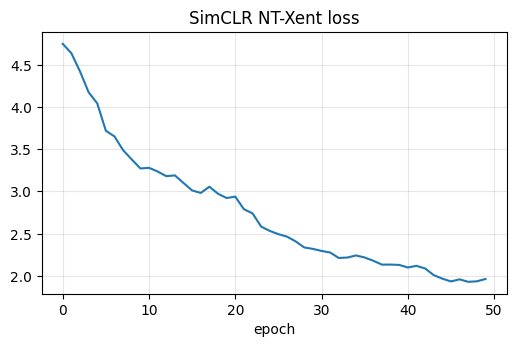
\includegraphics[width=0.49\columnwidth]{simclr_pretrain_loss.png}
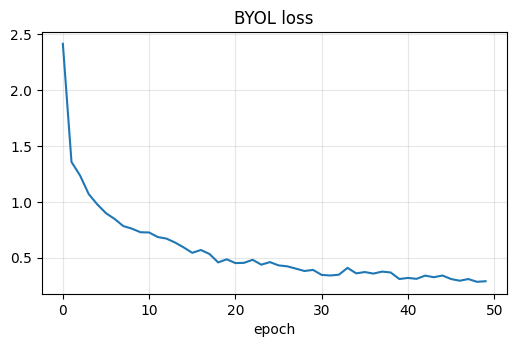
\includegraphics[width=0.49\columnwidth]{byol_pretrain_loss.png}\\[2pt]
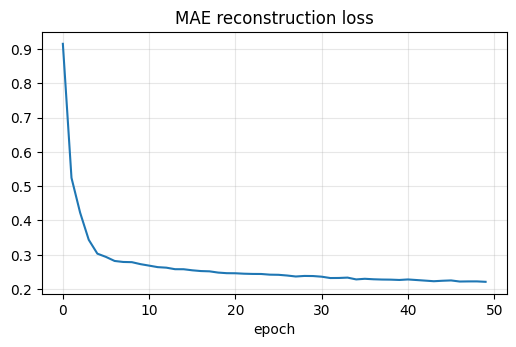
\includegraphics[width=0.49\columnwidth]{mae_pretrain_loss.png}
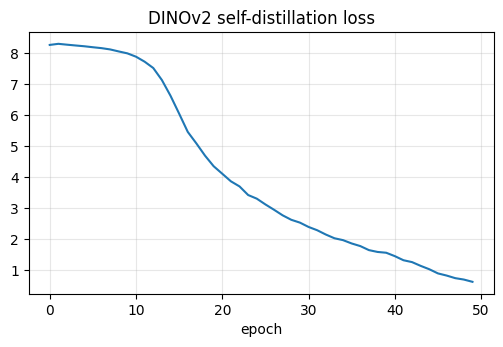
\includegraphics[width=0.49\columnwidth]{dinov2_pretrain_loss.png}
\caption{Pretext-task losses over 50 epochs. Top: SimCLR (NT-Xent), BYOL.
Bottom: MAE (masked reconstruction), DINOv2 (self-distillation).}
\label{fig:pretext}
\end{figure}

\begin{figure}[t]
\centering
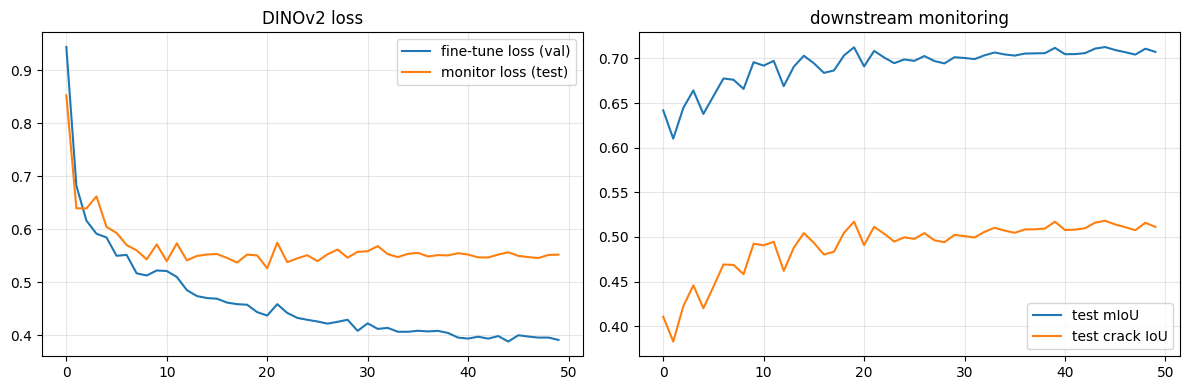
\includegraphics[width=\columnwidth]{dinov2_curves.png}
\caption{DINOv2 downstream fine-tuning. Left: loss on the labelled fine-tuning split
and on the monitored test split. Right: test-split mIoU and crack IoU per epoch.}
\label{fig:ftcurves}
\end{figure}

% ------------------------------------------------------------------ 6.6 RESULTS
\section{Results}

Table~\ref{tab:results} reports every Task-E metric on the held-out test split
alongside the Part-A fully-supervised baseline, and Fig.~\ref{fig:labeleff}
visualises the comparison.

\begin{table*}[t]
\caption{Test-set results. All Part-B rows are fine-tuned on \textbf{195} labelled
images ($21.5\%$ of the Part-A budget) at $224^2$; the Part-A baseline used
\textbf{909} labelled images at $512^2$. Best SSL value per column in bold.}
\label{tab:results}
\centering
\begin{tabular}{@{}llrrrrrrrr@{}}
\toprule
\textbf{Method} & \textbf{Backbone} & \textbf{Labels} &
\textbf{mIoU} & \textbf{IoU$_{\text{bg}}$} & \textbf{IoU$_{\text{crack}}$} &
\textbf{Pixel Acc.} & \textbf{Mean Pix. Acc.} & \textbf{Mean Dice} &
\textbf{\% of sup.} \\
\midrule
SimCLR (frozen)   & ResNet-50 & 195 & 0.6222 & 0.8672 & 0.3772 & 0.8771 & ---    & 0.7383 & 74.2 \\
SimCLR            & ResNet-50 & 195 & 0.6547 & 0.8810 & 0.4284 & 0.8908 & 0.8328 & 0.7683 & 78.1 \\
BYOL              & ResNet-50 & 195 & 0.6650 & 0.8837 & 0.4463 & 0.8937 & 0.8501 & 0.7777 & 79.3 \\
MAE               & ResNet-50 & 195 & 0.6971 & 0.9027 & 0.4915 & 0.9111 & 0.8609 & 0.8040 & 83.2 \\
\textbf{DINOv2}   & ViT-S/14  & 195 & \textbf{0.7128} & \textbf{0.9075} & \textbf{0.5181} &
                                       \textbf{0.9159} & \textbf{0.8819} & \textbf{0.8170} & \textbf{85.0} \\
\midrule
Part-A supervised (DeepLabV3-R50) & ResNet-50 & 909 & 0.8383 & 0.9562 & 0.7204 & 0.9607 & 0.9516 & 0.9076 & 100.0 \\
\bottomrule
\end{tabular}
\end{table*}

\begin{figure}[t]
\centering
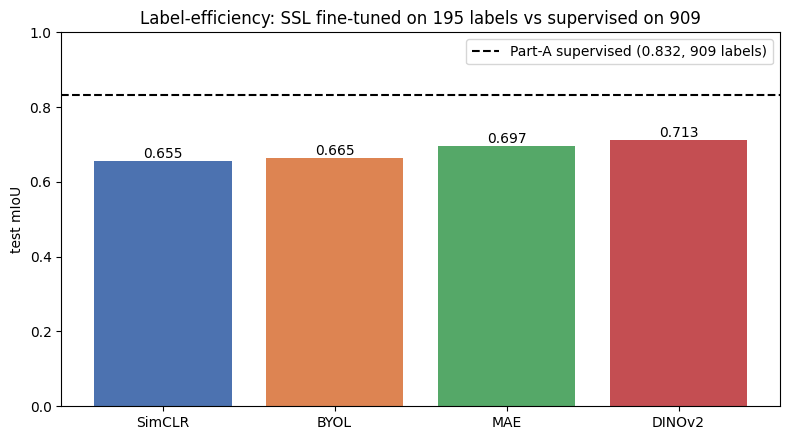
\includegraphics[width=\columnwidth]{final_label_efficiency.png}
\caption{Test mIoU of each self-supervised method (fine-tuned on 195 labels) against
the fully-supervised Part-A baseline (dashed, 909 labels).}
\label{fig:labeleff}
\end{figure}

The ordering is consistent across \emph{every} metric:
$\text{DINOv2} > \text{MAE} > \text{BYOL} > \text{SimCLR} > \text{SimCLR (frozen)}$.
The spread between the best and worst SSL configuration is $0.0906$ mIoU, which is
larger than the $0.0202$ mIoU that separated the three fully-supervised
architectures in Part~A --- i.e. \emph{the choice of pretext task mattered more here
than the choice of architecture did in Part~A}.

% ------------------------------------------------------------------ 6.7 ERROR
\section{Error Analysis}

\begin{figure}[t]
\centering
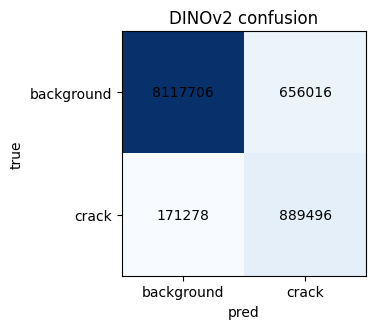
\includegraphics[width=0.49\columnwidth]{dinov2_confusion.png}
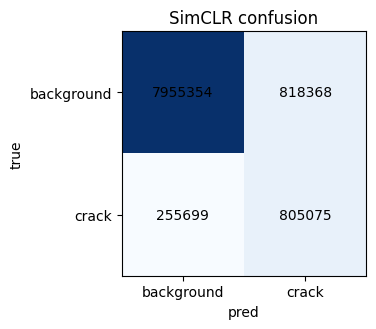
\includegraphics[width=0.49\columnwidth]{simclr_confusion.png}
\caption{Pixel-level confusion matrices for DINOv2 (left) and SimCLR (right).}
\label{fig:conf}
\end{figure}

\begin{figure}[t]
\centering
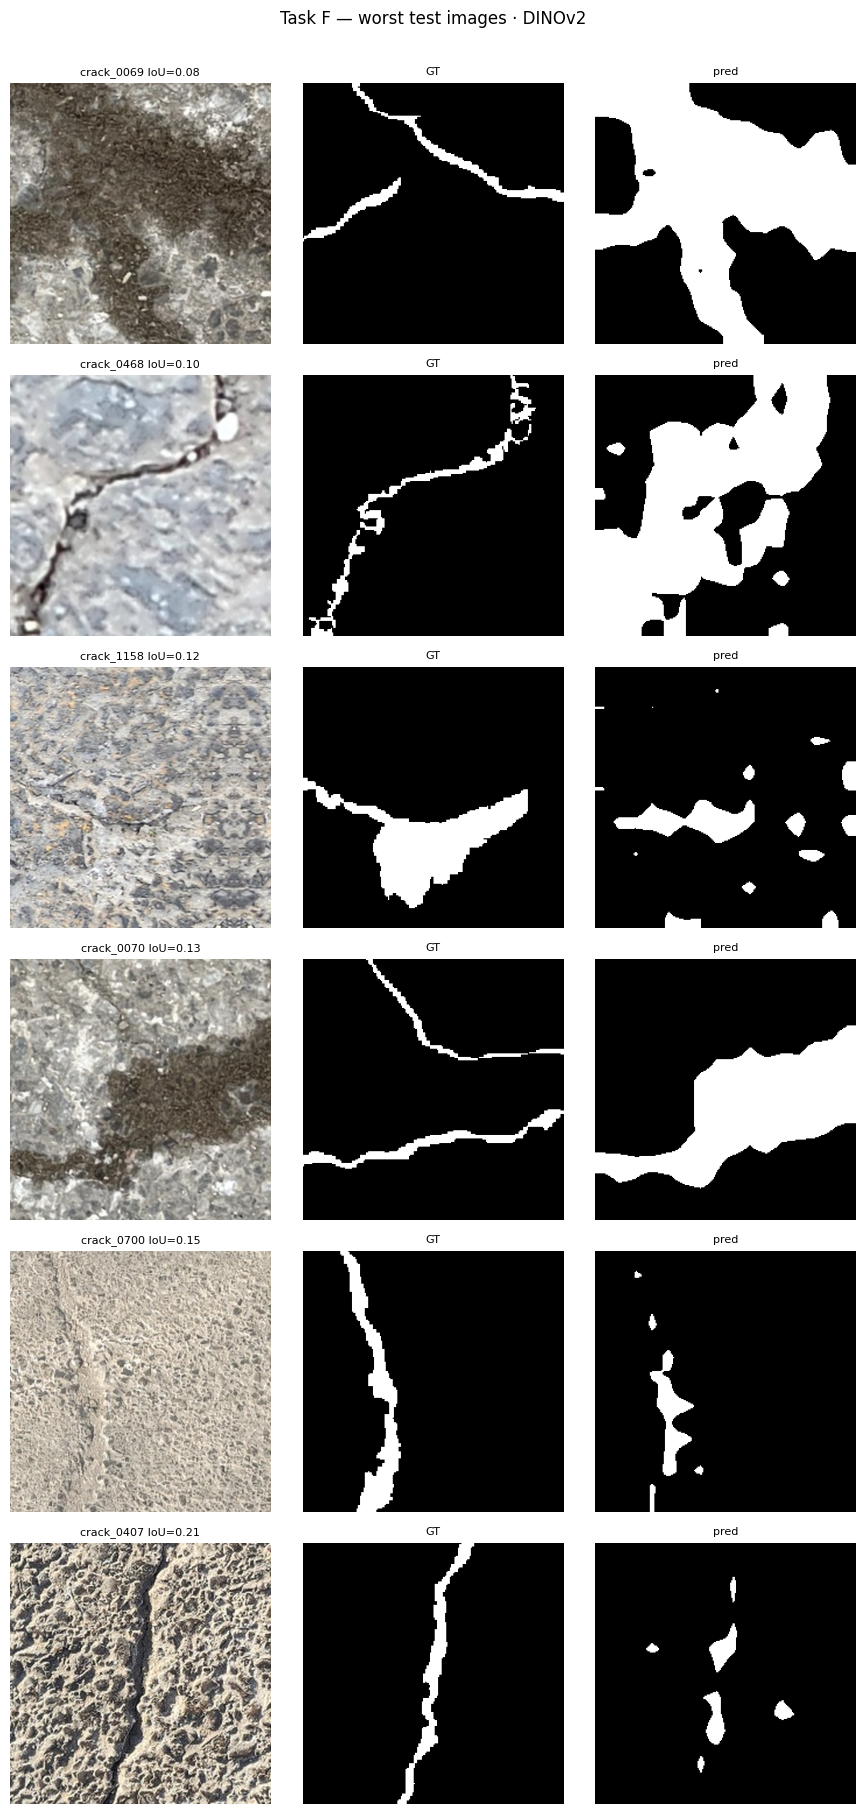
\includegraphics[width=0.85\columnwidth]{dinov2_worst.png}
\caption{Lowest-IoU test images for DINOv2: input, ground truth, prediction.}
\label{fig:worst}
\end{figure}

\subsection{Where the errors concentrate}
Errors are overwhelmingly concentrated in the \textbf{crack} class. Background IoU
never falls below $0.867$ and varies by only $0.040$ across all five configurations,
whereas crack IoU spans $0.377$--$0.518$ --- a relative spread of $37\%$. In other
words, every method has essentially solved the background class, and the entire
ranking in Table~\ref{tab:results} is decided by how well each encoder localises
cracks. This also explains why overall pixel accuracy is a poor summary here: because
cracks occupy only $\approx 11\%$ of pixels, a model can score $0.877$ pixel accuracy
(frozen SimCLR) while missing well over half the crack area.

\subsection{The dominant failure mode is over-segmentation}
Decomposing the confusion matrix into crack-class precision and recall
(Table~\ref{tab:pr}) shows that \emph{every} configuration is false-positive
dominant: recall ($0.76$--$0.84$) exceeds precision ($0.50$--$0.58$) by a wide
margin, so the models paint more crack than the ground truth contains. This is the
\emph{same} qualitative failure mode we reported for the fully-supervised models in
Part~A, and it is the expected consequence of the class-weighted loss
($w_{\text{crack}} = 4.63$), which deliberately trades precision for recall on the
minority class.

\begin{table}[t]
\caption{Crack-class precision and recall, reconstructed from the reported IoU,
pixel-accuracy and mean-pixel-accuracy figures (the reconstruction independently
recovers the ground-truth crack fraction as $10.79\%$, matching the dataset).
All configurations are false-positive dominant.}
\label{tab:pr}
\centering
\small
\begin{tabular}{@{}lrrr@{}}
\toprule
\textbf{Method} & \textbf{Recall} & \textbf{Precision} & \textbf{IoU$_{\text{crack}}$} \\
\midrule
SimCLR                  & 0.759 & 0.496 & 0.4284 \\
BYOL                    & 0.795 & 0.504 & 0.4463 \\
MAE                     & 0.797 & 0.562 & 0.4915 \\
DINOv2                  & 0.839 & 0.576 & 0.5181 \\
\midrule
Part-A DeepLabV3 (909 labels) & 0.940 & 0.755 & 0.7204 \\
\bottomrule
\end{tabular}
\end{table}

What \emph{does} change between the two parts is the severity, and it changes on both
axes at once: moving from the fully-supervised baseline to the best SSL model, recall
falls from $0.940$ to $0.839$ and precision falls from $0.755$ to $0.576$. Precision
therefore degrades proportionally more than recall ($-24\%$ against $-11\%$), which
tells us the reduced label budget costs the models \emph{boundary discipline} rather
than detection ability: they still find the cracks, but they draw them too thickly and
also respond to crack-like texture that is not annotated.

The gap between overall pixel accuracy and \emph{mean} pixel accuracy corroborates
this ordering. That gap is $0.058$ for SimCLR ($0.8908$ vs $0.8328$) and only $0.034$
for DINOv2 ($0.9159$ vs $0.8819$), shrinking monotonically as the methods improve;
since background recall is near-saturated, the shrinkage tracks the rise in crack
recall from $0.759$ to $0.839$. Note, however, that a low mean pixel accuracy does
\emph{not} by itself imply that false negatives dominate: because cracks occupy only
$\approx 11\%$ of pixels, false positives are drawn from a background pool roughly
nine times larger, so a model can have mediocre recall and still produce far more
false positives than false negatives --- which is exactly what
Table~\ref{tab:pr} shows.

\subsection{Which images fail, and how this compares to Part~A}
The lowest-IoU images in Fig.~\ref{fig:worst} are dominated by two recurring cases:
(i) very sparse hairline cracks, where a handful of mislabelled pixels destroys the
IoU of an image that contains almost no positive area, and (ii) low-contrast or
partially shadowed asphalt, where the crack boundary is genuinely ambiguous.

Part~A established quantitatively that its three architecturally distinct supervised
models failed on largely the \emph{same} images (per-image crack-IoU correlation
$0.89$--$0.94$; 12 of the 20 hardest images shared by all three), which we
interpreted as evidence that the residual difficulty is intrinsic to the data rather
than to any particular inductive bias. Qualitatively the Part-B failures point the
same way --- the hard cases are again thin, low-contrast, low-positive-area patches
--- and the final-comparison notebook reports the corresponding per-image correlation
and shared-worst-image overlap against the Part-A baseline directly. Two
Part-B--specific factors compound the problem. First, at $224^2$ a hairline crack that was three
pixels wide in Part~A is barely one pixel wide, so some ground-truth structure is
simply below the representable resolution. Second, none of the pretext tasks
supervises the encoder densely at the pixel level in a class-aware way, so fine
boundary precision has to be learned entirely from the 195 labelled images.

% ------------------------------------------------------------------ 6.8 LABEL EFF
\section{Label-Efficiency Discussion}

The central question was how much fully-supervised performance survives when the
label budget is cut to a fifth. With $195/909 = 21.5\%$ of the labels:

\begin{itemize}
  \item \textbf{DINOv2} recovers $85.0\%$ of the Part-A mIoU
        ($0.7128$ vs $0.8383$).
  \item \textbf{MAE} recovers $83.2\%$, \textbf{BYOL} $79.3\%$ and
        \textbf{SimCLR} $78.1\%$.
  \item The \textbf{frozen} SimCLR encoder recovers only $74.2\%$.
\end{itemize}

Ranked by label efficiency the order is
DINOv2 $>$ MAE $>$ BYOL $>$ SimCLR $>$ SimCLR (frozen).
Roughly $4.7\times$ fewer annotations cost about $15\%$ of relative mIoU for the best
method --- a favourable trade in any setting where annotation, not compute, is the
bottleneck.

Two qualifications must be attached to these numbers. First, as noted in
Section~II-C, Part~B runs at $224^2$ against Part~A's $512^2$, so an unknown portion
of the remaining $15\%$ is a resolution penalty on thin structures rather than a
label penalty; a matched-resolution rerun would be required to separate the two
effects cleanly. Second, the double role of the test split makes all Part-B numbers
mildly optimistic.

% ------------------------------------------------------------------ 6.9 INSIGHTS
\section{Insights}

\subsection{The ranking is not purely a comparison of pretext tasks}
The most important caveat about our own headline result is that DINOv2 is the only
method that began from a released checkpoint. SimCLR, BYOL and MAE were pretrained
\emph{from random initialisation} on 909 images, whereas DINOv2 inherited weights
learned from 142 million curated images and then received 50 further epochs of
in-domain self-distillation. Its victory therefore measures \emph{prior knowledge at
scale} at least as much as it measures the merit of self-distillation as a pretext
task. A scientifically clean comparison of the four objectives would require all four
to start from released checkpoints of the same scale, and we would present that as
the first correction to make in any follow-up.

\subsection{Dense pretext tasks suit dense downstream tasks}
The result we find genuinely instructive is MAE's. It reached mIoU $0.6971$ --- second
place, and within $0.016$ of DINOv2 --- after only \textbf{4.3 minutes} of
pretraining, roughly $7.6\times$ less compute than SimCLR's $32.9$ minutes, and it
did so from random initialisation. We attribute this to an alignment between the
pretext task and the downstream task. Masked reconstruction is a \emph{dense,
spatially local} objective: to inpaint a missing $16\times16$ patch of asphalt the
encoder must retain per-location texture information. Segmentation needs exactly
that. Contrastive objectives, by contrast, are \emph{image-level}: SimCLR and BYOL
compress an entire image to a single embedding and are explicitly trained to make
that embedding invariant to augmentation. Information that distinguishes one pixel
from its neighbour is not merely unnecessary for that objective --- it is actively
discarded.

\subsection{Contrastive augmentation may destroy the crack signal}
There is a domain-specific reason to expect contrastive learning to struggle on this
dataset in particular. A crack is a thin, low-contrast intensity variation on an
otherwise uniform grey surface. The standard SimCLR/BYOL augmentation pipeline
applies strong colour jitter and Gaussian blur and asks the network to become
\emph{invariant} to them. On natural images that discards nuisance lighting. On
pavement, contrast and fine high-frequency texture \emph{are} the signal, so the
pretext task is training away precisely the cues the segmenter later needs. A second,
more mundane factor is that contrastive learning depends on a large pool of
negatives; with a batch size of $64$ over $909$ images the pool is orders of
magnitude smaller than the setting these methods were designed for. Consistent with
this, negative-free BYOL outperformed SimCLR on every metric ($+0.0103$ mIoU), which
is what one expects when the negative pool is the weak link.

\subsection{Freezing hurt --- and that is itself a measurement}
Linear-probing the frozen SimCLR encoder reached mIoU $0.6222$ against $0.6547$ when
fine-tuned, a gap of $0.0325$. We read this in two directions. The frozen encoder
still recovered $74.2\%$ of the fully-supervised baseline, so 50 epochs of contrastive
pretraining on 909 unlabelled images did learn genuinely useful structure --- this is
not noise. But the fact that a third of a mIoU point was recoverable simply by
unfreezing indicates the representation was not yet \emph{linearly} usable for dense
prediction. Had the gap been near zero we could have claimed the pretext task
produced directly transferable features; had it been very large we would suspect the
features were nearly useless and the decoder was doing all the work. The moderate gap
we measured places SimCLR-on-909-images in between, and justifies our decision to
fine-tune the remaining three methods.

\subsection{Encoder pretraining mattered more than architecture did}
Comparing the two parts of this project is revealing. In Part~A, three
architecturally very different supervised segmenters --- a CNN with ASPP, a
hierarchical transformer, and a real-time detector adapted to dense output ---
finished within $0.0202$ mIoU of one another. In Part~B, holding the decoder fixed
and changing only the pretext task produced a spread of $0.0906$ mIoU, roughly
$4.5\times$ larger. With abundant labels, the architecture is close to irrelevant;
in the low-label regime, how the encoder was pretrained dominates. If we had to
allocate effort on a new dataset with few labels, this argues for spending it on the
representation rather than on decoder search.

\subsection{What we would do next}
With a larger compute budget we would, in order: (i) rerun Part~B at
$448\times448$ or $512\times512$ to remove the resolution confound and isolate the
true label-efficiency effect --- for a ViT-S/14 encoder $448$ is the natural choice
since $448/14 = 32$ gives a clean token grid; (ii) initialise SimCLR, BYOL and MAE
from released ImageNet SSL checkpoints so that all four methods are compared on equal
footing; (iii) replace the image-level contrastive objectives with a
\emph{dense} contrastive method such as DenseCL or PixPro, which match features at
the pixel or region level and are designed for exactly this downstream task; and
(iv) extend pretraining well beyond 50 epochs, since none of our pretext losses had
plateaued --- SimCLR was still descending ($1.97$ at epoch 50) when the budget ran
out, so 50 epochs is a floor imposed by the assignment rather than a converged model.

\subsection{What surprised us}
Two things. First, the sheer efficiency of MAE: we expected reconstruction to need
long training to become useful, yet it delivered second place from $4.3$ minutes of
pretraining, which suggests that on a texture-dominated, single-foreground-class
dataset the reconstruction signal is unusually informative per unit of compute.

Second, \emph{which} component of the error grew when we cut the label budget. Our
initial expectation was that fewer labels would make the models cautious and cause
them to miss cracks. The decomposition in Table~\ref{tab:pr} shows the opposite:
every SSL model remains false-positive dominant, just as the supervised models were,
and precision degrades proportionally more than recall ($-24\%$ versus $-11\%$
relative to the Part-A baseline). Fewer labels did not make the models blind to
cracks --- they still recover $84\%$ of crack pixels --- it made them \emph{imprecise
about where a crack stops}. In hindsight this is consistent with how the two error
types are bounded: false negatives are capped by the small crack area, whereas false
positives can be drawn from a background pool nine times larger, so boundary
sloppiness is punished asymmetrically. For a practical inspection system this is
arguably the better failure mode --- an inflated crack mask is easier to post-process
than a missed crack --- but it means IoU understates how well these models actually
localise damage.

% ------------------------------------------------------------------ 6.10 CONCL
\section{Conclusion}

We replaced the supervised encoder of our best Part-A segmenter with four
self-supervised alternatives and fine-tuned each on only $21.5\%$ of the original
labels. The best configuration, DINOv2 with a token-to-grid adapter feeding a
DeepLabV3 ASPP head, reached mIoU $0.7128$ --- $85.0\%$ of the fully-supervised
result --- and the ordering DINOv2 $>$ MAE $>$ BYOL $>$ SimCLR held across every
metric. A frozen encoder consistently underperformed a fine-tuned one, indicating
that representations learned from 909 in-domain images still require adaptation for
dense prediction. Self-supervision is therefore a practical answer to annotation
scarcity in pavement inspection, though the residual gap --- part label budget, part
input resolution --- shows it is not yet a free substitute for supervision.

% ------------------------------------------------------------------ REFERENCES
\begin{thebibliography}{9}
\bibitem{simclr} T.~Chen, S.~Kornblith, M.~Norouzi and G.~Hinton,
``A Simple Framework for Contrastive Learning of Visual Representations,''
in \emph{Proc. ICML}, 2020.

\bibitem{byol} J.-B.~Grill \emph{et al.},
``Bootstrap Your Own Latent: A New Approach to Self-Supervised Learning,''
in \emph{Proc. NeurIPS}, 2020.

\bibitem{mae} K.~He, X.~Chen, S.~Xie, Y.~Li, P.~Doll\'ar and R.~Girshick,
``Masked Autoencoders Are Scalable Vision Learners,''
in \emph{Proc. CVPR}, 2022.

\bibitem{dinov2} M.~Oquab \emph{et al.},
``DINOv2: Learning Robust Visual Features without Supervision,''
\emph{arXiv:2304.07193}, 2023.

\bibitem{dino} M.~Caron \emph{et al.},
``Emerging Properties in Self-Supervised Vision Transformers,''
in \emph{Proc. ICCV}, 2021.

\bibitem{deeplab} L.-C.~Chen, G.~Papandreou, F.~Schroff and H.~Adam,
``Rethinking Atrous Convolution for Semantic Image Segmentation,''
\emph{arXiv:1706.05587}, 2017.

\bibitem{pavecrack} M.~Mahi, ``PaveCrack1300: A UAV-Acquired Pavement Crack
Segmentation Dataset,'' Mendeley Data, DOI: 10.17632/8b27pdcxv7, 2026. CC BY 4.0.

\bibitem{torchvision} PyTorch, ``torchvision DeepLabV3 documentation.''
\url{https://pytorch.org/vision/stable/models/deeplabv3.html}

\bibitem{hf} HuggingFace, ``DINOv2 model documentation.''
\url{https://huggingface.co/docs/transformers/model_doc/dinov2}
\end{thebibliography}

\end{document}
